\chapter{Deep Learning}

\section{Introduction }
L’apprentissage profond ou le deep Learning est un nouveau domaine de recherche du Machine Learning(ML), qui a été introduit dans le but de rapprocher le ML de son objectif principal : l’intelligence artificielle.
 Il concerne les algorithmes inspirés par la structure et le fonctionnement du cerveau. 
 Ils peuvent apprendre plusieurs niveaux de représentation dans le but de modéliser des relations complexes entre les données.
 
 \begin{figure}[h]
\centering
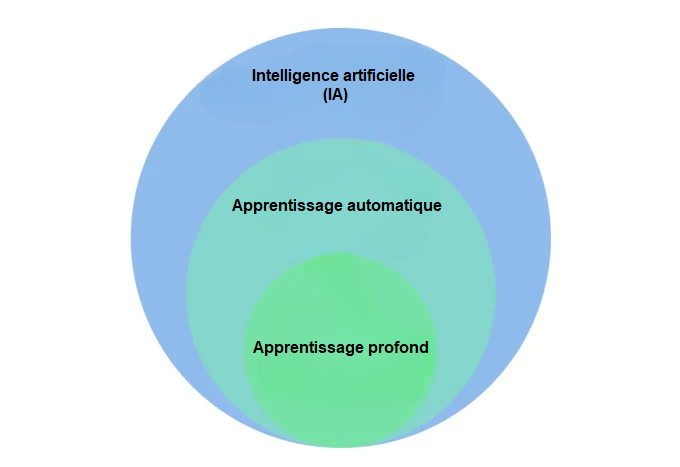
\includegraphics[scale=0.9]{Images/ia reglo.png}
\caption{La relation entre l’intelligence artificielle, le Machine L earning et le deep learning.}
\label{fig:08}
\end{figure} 
 
 \section{L’apprentissage profond }
 L'apprentissage profond est une technologie d'intelligence artificielle révolutionnaire qui permet aux machines d'apprendre à partir de données massives, ouvrant ainsi la voie à des avancées majeures. Malgré ses succès, il présente des défis, mais continue de repousser les frontières de l'intelligence artificielle.
 
\subsection{Définition l'apprentissage profond}
L’apprentissage profond en anglais cet appelée «Deep Learning » une technique d'apprentissage automatique révolutionnaire qui a permis de réaliser des progrès importants dans de nombreux domaines tels que la vision par ordinateur, la reconnaissance de la parole et la traduction automatique. 
Grâce à sa capacité à apprendre par elle-même et à résoudre des problèmes complexes, l'apprentissage profond est un outil puissant qui continuera à jouer un rôle majeur dans l'évolution de l'intelligence artificielle. 

\subsection{Domaines d'application de l'apprentissage profonde }
Le deep Learning utilisé dans plusieurs domaines différents tels que :

\begin{itemize}
\item  \textbf{Traitement du langage naturel (NLP)} : L'apprentissage profond est employé dans la compréhension du langage naturel, la traduction automatique, la génération de texte, la classification de texte, et l'analyse des sentiments.

\item \textbf{Santé} : L'apprentissage profond est appliqué dans le diagnostic médical, la segmentation d'images médicales, la prédiction de maladies, et la découverte de médicaments.

\item \textbf{Vision par ordinateur} : L'apprentissage profond est largement utilisé pour la reconnaissance d'images, la segmentation d'images, la détection d'objets, la classification d'images, et la génération d'images.

\item \textbf{Robotique} : L'apprentissage profond est employé dans la perception sensorielle des robots, la planification de mouvements, et l'interaction homme-robot.
\end{itemize}

 \section{Principes de fonctionnement }
 D’apprentissage en profondeur sont formés sur la base des structures de données complexes qu'ils rencontrent. 
Ils construisent des modèles informatiques composés de plusieurs couches (couche d'entrée, couche cachée, couche de sortie) de traitement pour créer plusieurs niveaux d'abstraction pour représenter les données. 

\begin{figure}[h]
\centering
\includegraphics[scale=0.8]{Images/réseau.png}
\caption{les couches d’apprentissage profond.}
\label{fig:09}
\end{figure}

\subsection{Les types des couches dans d’apprentissage profond}

\begin{itemize}
\item  \textbf{Couche d’entrée} : composée d’un ensemble de neurones qui favoriseront la propagation des informations dans le réseau neuronal. Elle comprend un nombre de neurones généralement égal au nombre de caractéristiques constituant l’enregistrement en entrée (p. ex. une image, une transaction, etc.).
\item \textbf{Couches intermédiaires} : servant à traiter l’information propagée dans le réseau de neurones pour capturer les caractéristiques de son apprentissage.
\item \textbf{Couche de sortie} : formée d’un ensemble de neurones représentant les différentes classes de résultat.
 Dans une problématique de classification, les classes sont les différentes possibilités que le résultat peut offrir.
 
\end{itemize}

 \section{Les poids }
 \label{Les poids}
 Les poids des flèches sont utilisés pour accorder de l'importance à certaines fonctionnalités par rapport à d'autres, afin d'obtenir les résultats souhaités. La somme pondérée de tous les poids des flèches est calculée pour chaque neurone d'une couche cachée, et chacun de ces neurones exécute une fonction d'activation qui lui est propre.

 \section{La fonction d'activation }
 Une fonction d’activation, qui associe à chaque valeur agrégée une unique valeur de sortie dépendant du seuil.
 
 \begin{figure}[h]
\centering
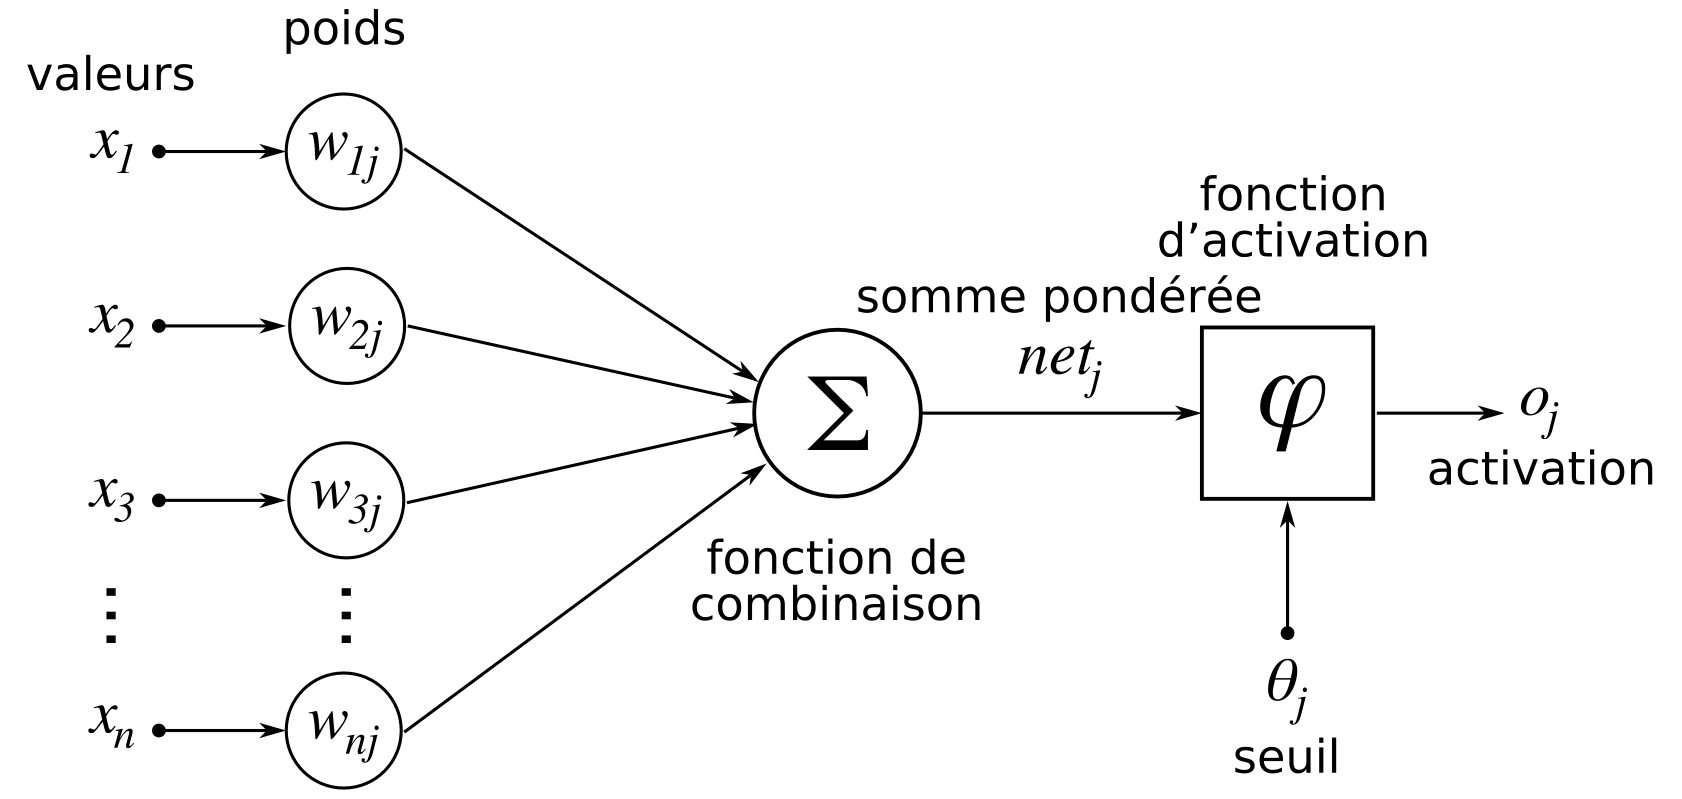
\includegraphics[scale=0.3]{Images/1-neurone-formel.png}
\caption{Fonction d’activation.}
\label{fig:10}
\end{figure}

\subsection{La fonction Relu }

La fonction Unité Linéaire Rectifiée en anglais, appelée Rectified Linear Unit (ReLU), est la fonction d'activation la plus couramment utilisée en Deep Learning. Elle est définie comme suit :

\[ \text{ReLU}(x) = \max(x, 0) \]

Cette fonction renvoie $x$ si $x$ est supérieur à 0, et 0 sinon. Autrement dit, elle calcule le maximum entre $x$ et 0.


\begin{figure}[h]
\centering
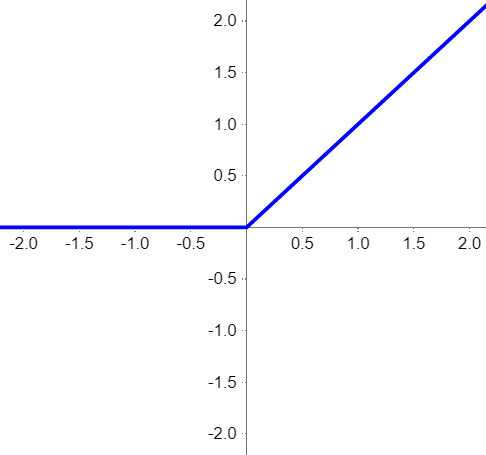
\includegraphics[scale=0.5]{Images/relu.png}
\caption{La fonction Relu.}
\label{fig:11}
\end{figure}

Cette fonction permet d’appliquer un filtre en sortie de couche. 
Elle laisse passer les valeurs positives dans les couches suivantes et bloque les valeurs négatives. 
Ce filtre permet alors au modèle de se concentrer uniquement sur certaines caractéristiques des données, les autres étant éliminées.

\subsection{La fonction d'un softmax }
La fonction Softmax est la fonction d'activation utilisée en dernière couche d'un réseau de neurones construit pour effectuer une tâche de classification multi-classes. Pour chaque sortie, Softmax donne un résultat entre 0 et 1. De plus, si l'on additionne ces sorties entre elles, le résultat donne 1.

La fonction Softmax est définie mathématiquement comme suit :

\[ \text{Softmax}(x) = \frac{e^{x}}{\sum_{i} e^{x_i}} \]


\begin{figure}[h]
\centering
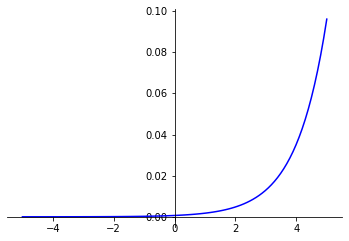
\includegraphics[scale=0.5]{Images/Softmax.png}
\caption{La fonction d'un softmax.}
\label{fig:12}
\end{figure}

La fonction Softmax, grâce à sa caractéristique de produire des résultats qui, additionnés, donnent 1, respecte les lois de probabilité. Elle est donc le noyau dur d’un réseau de neurones construit pour effectuer une tâche de classification multi-classes.

\subsection{La fonction sigmoïde }
La fonction sigmoïde est la fonction d'activation utilisée en dernière couche d'un réseau de neurones construit pour effectuer une tâche de classification binaire. Elle donne une valeur entre 0 et 1.

La fonction sigmoïde est définie mathématiquement comme suit :

\[ \text{Sigmoid}(x) = \frac{1}{1 + e^{-x}}\]
\begin{figure}[h]
\centering
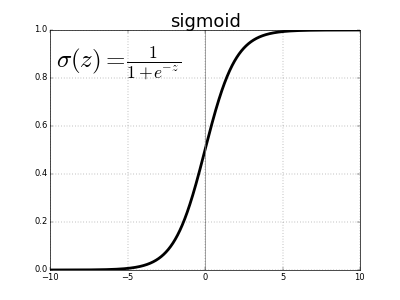
\includegraphics[scale=0.5]{Images/sigmoid.png}
\caption{La fonction sigmoïde.}
\label{fig:13}
\end{figure}

Cette valeur peut être interprétée comme une probabilité. Dans une classification binaire, la fonction d’activation sigmoïde permet alors d’obtenir, pour une donnée, la probabilité d’appartenir à une classe.
Dans cet exemple, plus le résultat de la sigmoïde est proche de 1, plus le modèle considère que la critique est positive. Inversement, plus le résultat de la sigmoïde est proche de 0, plus le modèle considère que la critique est négative.
La fonction d’activation sigmoïde permet donc d’obtenir un résultat ambivalent, donnant une indication sur deux classes à la fois.

\section{Les différents types de model deep Learning}
On va présenter dans cette section les modèles de deep Learning utilisés dans notre proposition à savoir les CNN, RNN, LSTM et ANN.

\subsection{Le réseau de neurone convolutif (CNN) }
Le nom ‘Réseau de neurones à convolution’ indique que le réseau emploi une opération mathématique appelée la convolution.
 Les réseaux de convolution sont un type spécialisé de réseaux neuronaux qui utilisent la convolution à la place de la multiplication matricielle générale dans au moins une de leurs couches.
 Les CNN sont l’un des meilleurs algorithmes d’apprentissage pour faire l’opération de convolution qui aide à l’extraction de fonctionnalités utiles à partir de points de données corrélés localement.
 La sortie des noyaux convolutifs est ensuite affectée à l’unité de traitement non linéaire (fonction d’activation), qui non seulement aide à apprendre les abstractions, mais intègre également la non-linéarité dans l’espace des fonctionnalités.

\begin{figure}[!h]
\centering
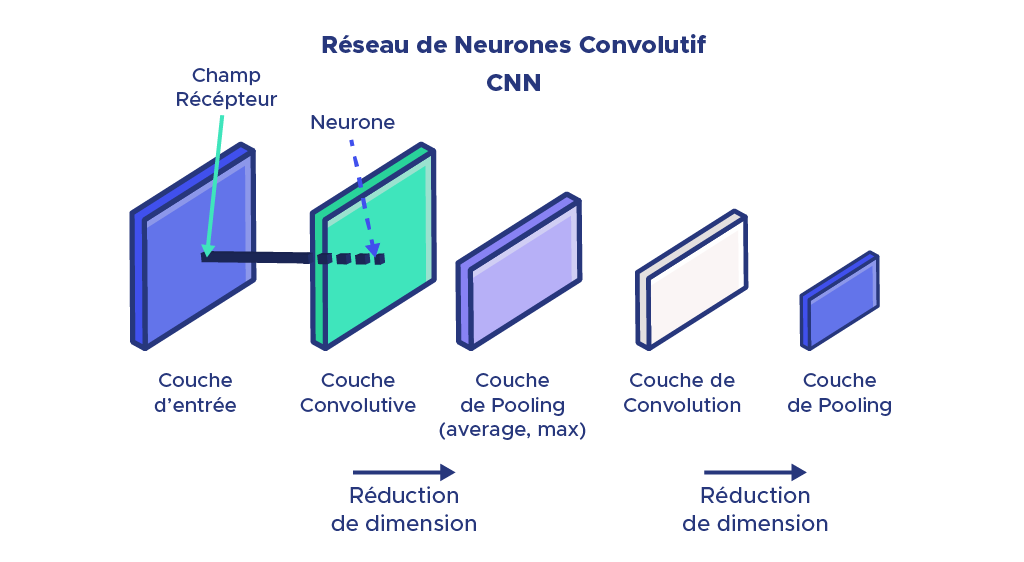
\includegraphics[width=13cm, height=6cm]{Images/illu_DenseNet-09.png}
\caption{Structure générale d’un réseau CNN.}
\label{fig:14}
\end{figure}
\newpage
\subsection{Réseau de neurones récurrents (RNN) }
Un réseau de neurones récurrent (RNN, Recurrent Neural Network) est un type de réseau de neurones artificiels principalement utilisé dans la reconnaissance vocale et le traitement automatique du langage naturel et la traduction automatique.
Les RNN sont conçus de manière à reconnaître les caractéristiques séquentielles et les modèles d'utilisation des données requis pour prédire les scénarios faisant intervenir le contexte dans la prédiction d'un résultat . 

\begin{figure}[!h]
\centering
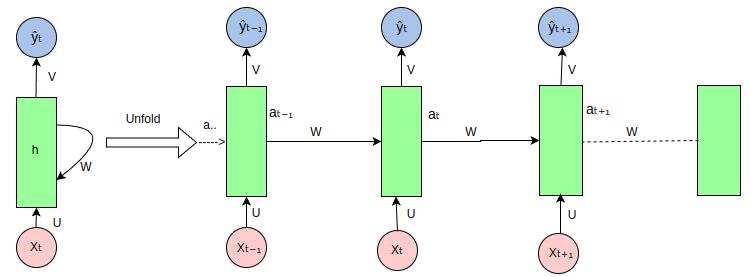
\includegraphics[scale=0.6]{Images/1_dznTsiaHCvRc70fxWWEcgw.png}
\caption{Architecture de RNN.}
\label{fig:15}
\end{figure}
\newpage
\subsection{Les réseaux LSTM }
Les réseaux mémoire à long terme (LSTM : Long Short-Term Memory, en anglais) sont des dérivés de RNN. Ils peuvent apprendre et mémoriser des dépendances sur une longue durée. Les LSTM conservent ainsi les informations mémorisées sur le long terme. Ils sont particulièrement utiles pour prédire des séries chronologiques, car ils se rappellent des entrées précédentes. Outre ce cas d'utilisation, les LSTM sont également utilisés pour composer des notes de musique et reconnaître des voix.

\begin{figure}[!h]
\centering
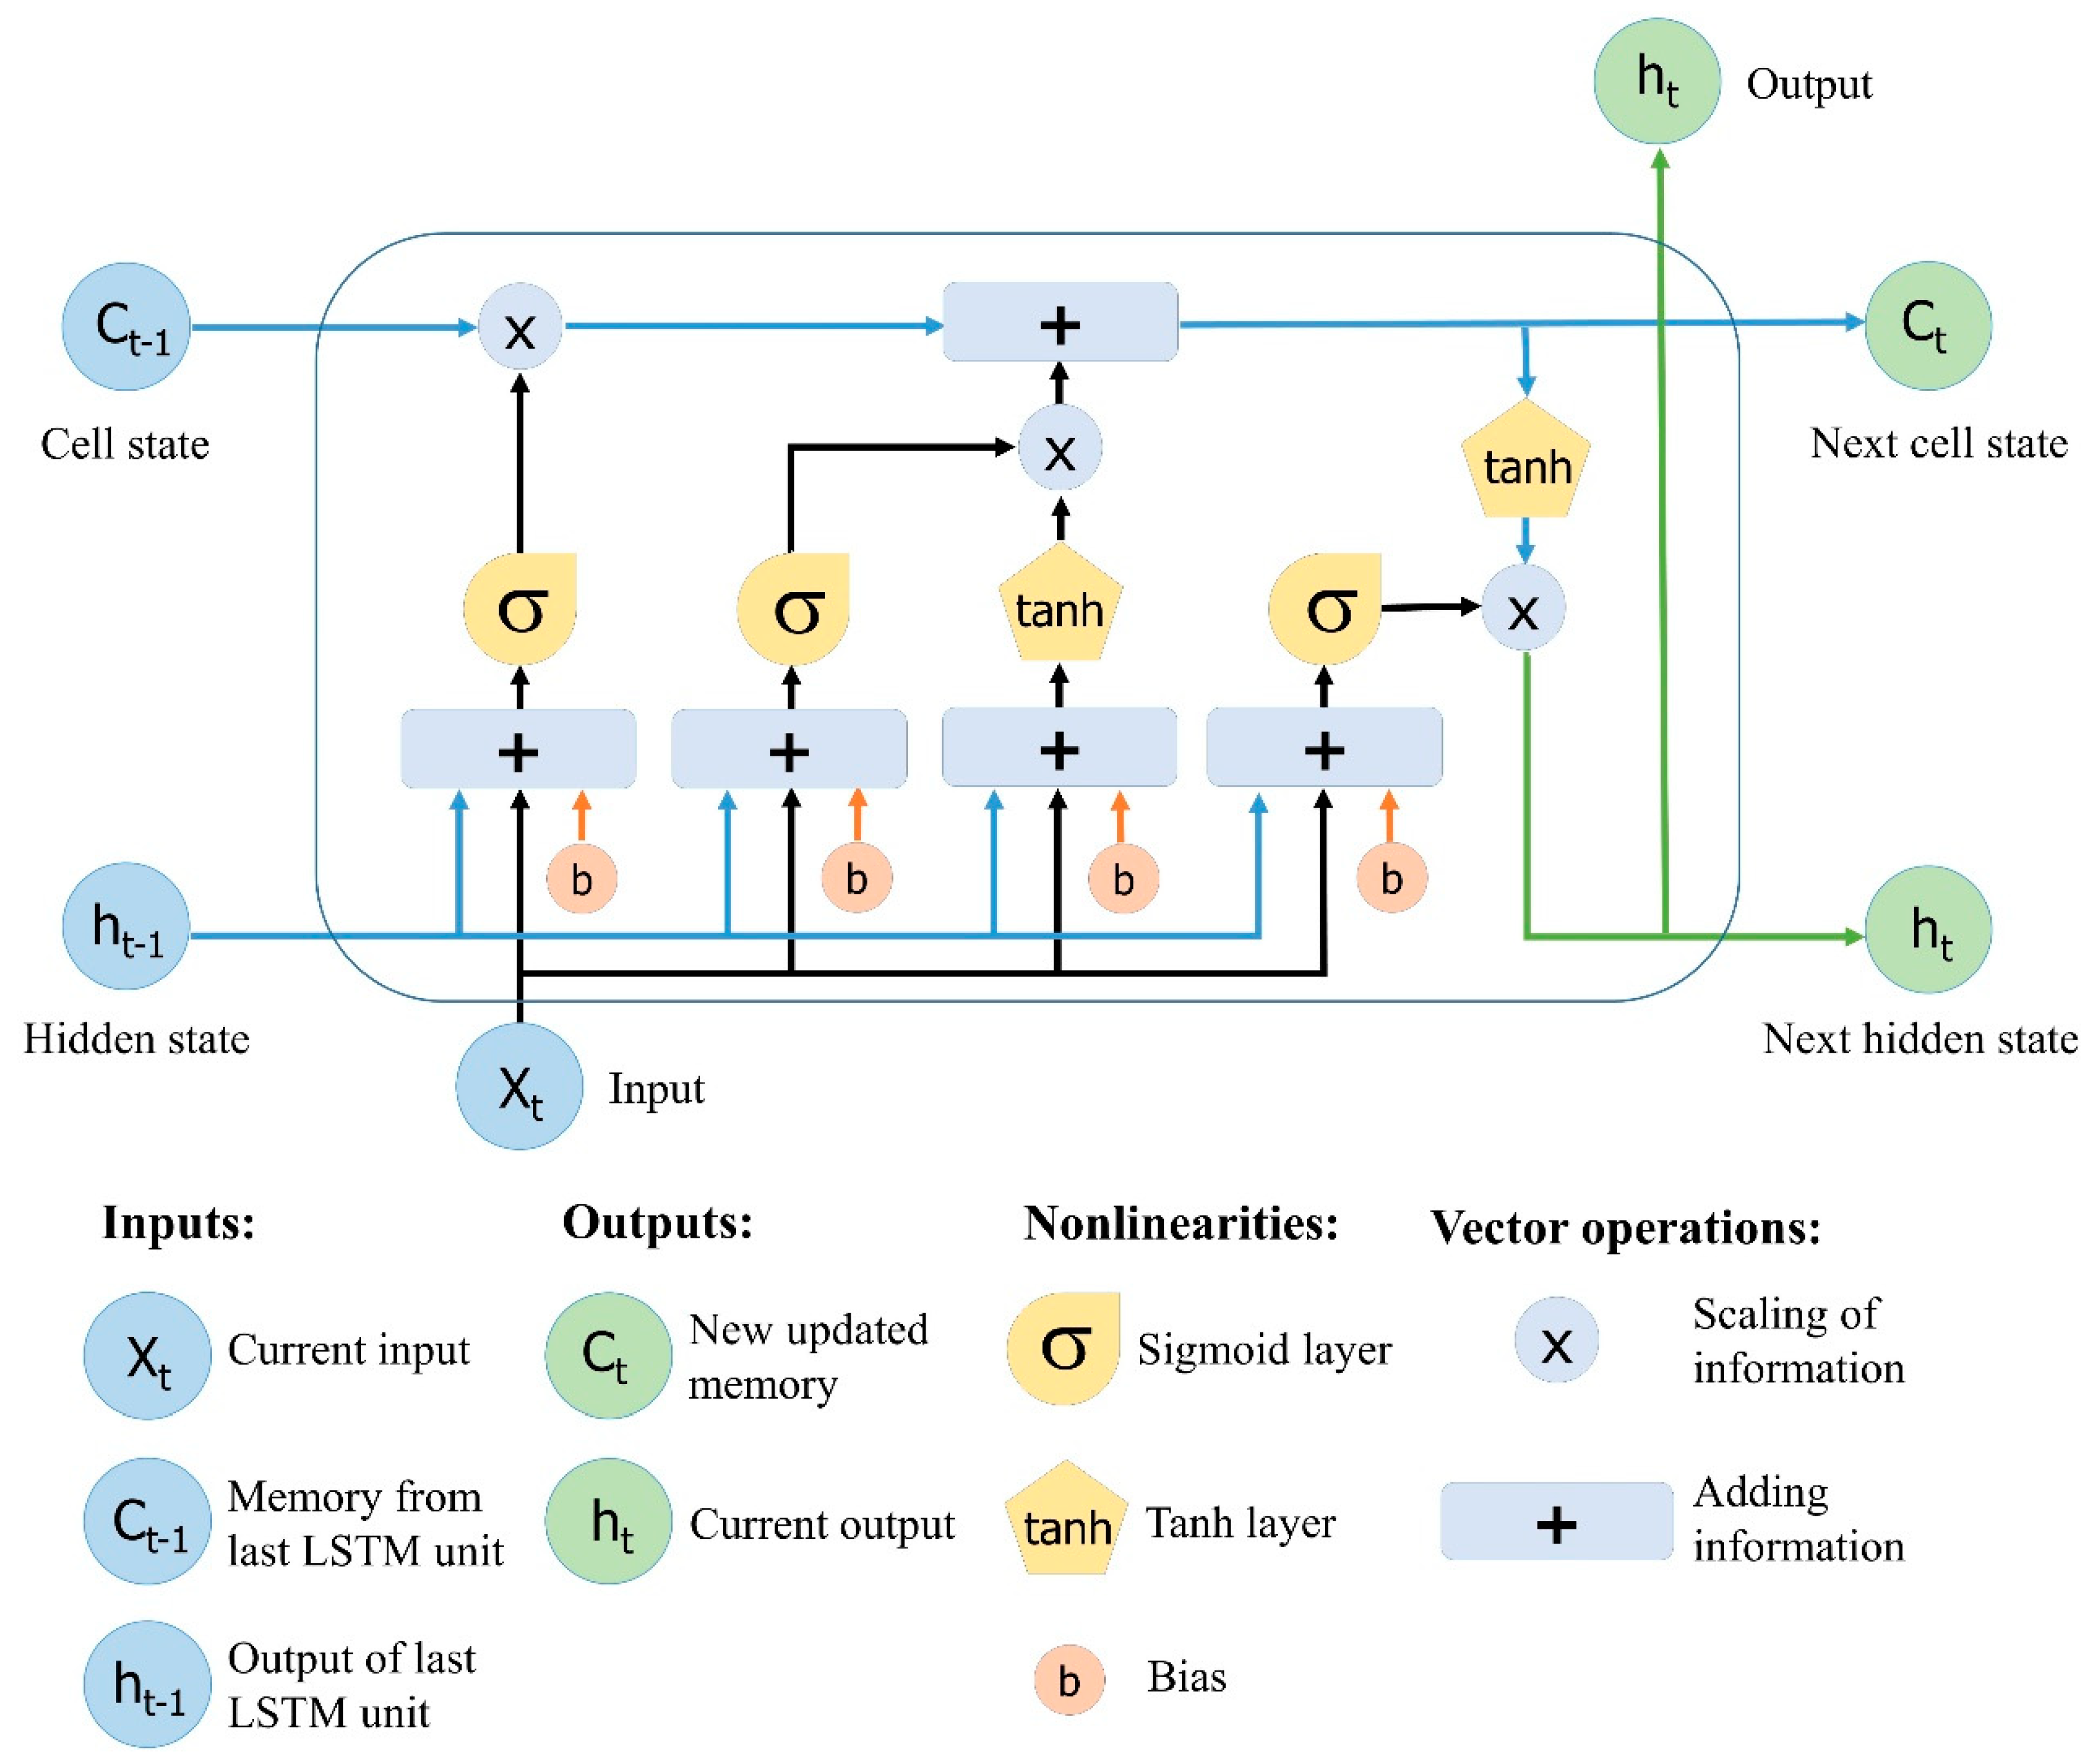
\includegraphics[scale=0.1]{Images/water-11-01387-g004.png}
\caption{Le module répétitif dans un LSTM.}
\label{fig:16}
\end{figure}
\newpage
\subsection{Réseaux de neurones artificiel (ANN) }
C’est une structure constituée de suite successive de couches de nœuds et qui permet de définir une fonction de transformation non linéaire des vecteurs d’entrées (composés dans le cas de classification des mots pondérés de leur poids) en vecteur de catégories. 
 La disposition des neurones dans le réseau ainsi que le nombre de couches utilisées ont une influence sur le résultat de classification.
Comparés aux autres méthodes de classification par apprentissage supervisé, les réseaux de neurones artificiels sont habituellement utilisés pour des tâches de classification. 
Par analogie avec la biologie, ces unités sont appelées neurones formels.
Un neurone formel est caractérisé par :

\begin{itemize}
\item Le type des entrées et des sorties.
\item Une fonction d’entrée.
\item Une fonction de sortie.
\end{itemize}

\begin{figure}[!h]
\centering
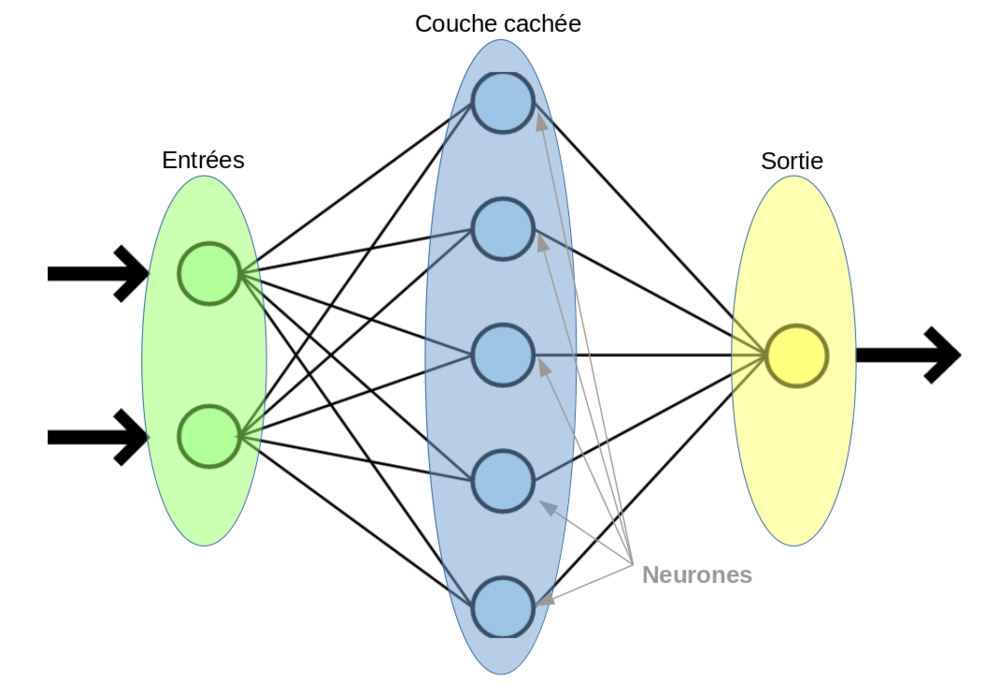
\includegraphics[scale=0.3]{Images/ANN.png}
\caption{Architecture de réseau de neurones artificiels.}
\label{fig:17}
\end{figure}

\newpage
\section{ Conclusion }

Dans ce chapitre nous avons présenté l'apprentissage en profondeur (DL) et ses différents types de réseaux de neurones artificiels : les réseaux de neurones artificiels (ANN), les réseaux de neurones convolutifs (CNN) et les réseaux de neurones récurrents (RNN), y compris les réseaux à mémoire longue durée (LSTM).

Le chapitre suivant se concentre sur l'expérimentation de la construction de modèles de réseaux de neurones artificiels avec compression de données utilisant l'algorithme des composantes principales (PCA). 
Nous appliquerons également différents types d'algorithmes d'optimisation.


